
\documentclass[
12pt,
a4paper,
bibliography=totocnumbered, %Literaturverzereichnis als Eintrag ins Inhaltsverzeichnis
%twoside, %Zweiseitiger Druck
BCOR=1cm, %Platz zum Lochen
oneside, %Einseitiger Druck
]{scrartcl}

\usepackage{geometry}

\usepackage[default]{fontsetup}
%\usepackage[onehalfspacing]{setspace}

\usepackage[ngerman]{babel}
\usepackage[babel=true,german=quotes]{csquotes}

\usepackage{microtype}
\usepackage{mleftright}
%\newcommand{\Le}{\mleft}
%\newcommand{\Ri}{\mright}
\usepackage[no-script, no-scriptscript, no-inner, no-close]{innerscript}

% Mathepakete (unicode-math ersetzt amssymb, amsfonts etc.)
\usepackage{amsmath,amsthm}
\usepackage{mathtools}
\usepackage{fixdif,derivative}
\usepackage{physics2}
\usephysicsmodule{ab.legacy}

\usepackage{unicode-math}
\setmathfont{NewCMMath-Book}
\setmathfont{NewCMMath-Book}[range=cal, StylisticSet=1]
\setmathfont{NewCMMath-Book}[range=scr]

\usepackage{siunitx}
\sisetup{detect-weight=true, detect-family=true,locale=DE,range-phrase={\,bis\,},list-final-separator ={\,\linebreak[0] \text{und}\,},separate-uncertainty=true,per-mode = symbol-or-fraction}
%\SI[per-mode = fraction]{1}{\meter\per\second} erzwingt auch im Fließtext die Bruchdarstellung.
\DeclareSIUnit\curie{Ci}%Zusätzliche Einheit definieren

\usepackage{tabularx, booktabs, multirow}
\usepackage{array}
\usepackage{enumitem}
\usepackage{float}
\usepackage{graphicx}
\usepackage{xurl}

\usepackage[final]{pdfpages}
\usepackage{framed, color} %Framed: Paket, mittels dessen ein Rahmen um einen Bereich definiert werden kann. Color: Lässt Farbdarstellung in Schrift, Hintergrund etc. zu

\usepackage{scrlayer-scrpage} %Header für die KOMA-script-Klasse

%\usepackage[square,numbers]{natbib}
\usepackage{subfigure} %Mehrere Bilder in einer Figure-Umgebung

\usepackage[bookmarks,colorlinks=true]{hyperref}
\hypersetup{
	colorlinks,
	linktocpage,
	citecolor=black,
	filecolor=black,
	linkcolor=black,
	urlcolor=black,
	pdftitle=X,
	pdfauthor=JM-VS
}

\usepackage[backend=biber, style=chem-angew]{biblatex}
\addbibresource{lit.bib}

\numberwithin{equation}{section} % Die Nummerierung von Gleichungen bekommt die jeweilige Section-Nummer als Präfix

\setlength{\parindent}{0pt} %Einrücktiefe von neuen Absätzen
\setlength{\parskip}{6pt} %Abstand von Absätzen

\pagestyle{scrheadings}%Kopf und Fußzeilen
\ohead{\textbf{\GRUPPENNR\ - \VERSUCHSNR}} %Header oben links auf linker Seite (ungerade Seitenzahl) und oben rechts auf rechter Seite (gerade Seitenzahl), beinhaltet gruppennummer und Versuchskürzel. Im Fall eine einseitigen Dokuments: Header oben rechts
\ihead{\VerfasserEINS\;\&\;\VerfasserZWEI} %Header oben rechts auf linker Seite und oben links auf rechter Seite. Beinhaltet die Namen der Verfasser. Im Fall eine einseitigen Dokuments: Header oben links!
\ofoot{\thepage} %Footer unten links auf linker und unten rechts auf rechter Seite, enthält die jeweilige Seitenzahl. Im Fall eines einseitigen Elements: Footer unten rechts!
\cfoot{\empty} %Mittig unten im Footer soll nichts eingetragen werden
\ifoot{\empty} %Footer unten rechts auf linker und unten links auf rechter Seite. Hier ebenfalls leer.

\newcommand{\tz}{T_{\text{II}}}
\newcommand{\ts}{T_{\text{S}}}
\newcommand{\tgl}{T_{\text{gl}}}
\newcommand{\tgeg}{T_{\text{geg}}}
\newcommand{\omz}{\omega_{\text{II}}}
\newcommand{\omgl}{\omega_{\text{gl}}}
\newcommand{\omgeg}{\omega_{\text{geg}}}
\newcommand{\kB}{k_{\text{B}}}

% Hier können die individuellen Anpassungen vorgenommen werden, die sich auf das Titelblatt und die Kopfzeilen auswirken.

\newcommand{\VERSUCHSDATUM}{24.09.2025}
\newcommand{\PROTOKOLLDATUM}{\today}

\newcommand{\VerfasserEINS}{Julian Molt}
\newcommand{\MatNoEINS}{3803097}
\newcommand{\StudiengangEINS}{Physik}

\newcommand{\VerfasserZWEI}{Valentin Stopper}
\newcommand{\MatNoZWEI}{3774391}
\newcommand{\StudiengangZWEI}{Physik}

\newcommand{\BETREUER}{Lara Zaiser}
\newcommand{\GRUPPENNR}{A-016}

\newcommand{\VERSUCHSNR}{M23}
\newcommand{\VERSUCHSNAME}{Gekoppelte Pendel}

\newcommand{\lh}{\ell_{\mathrm{H}}}
\newcommand{\ls}{\ell_{\mathrm{S}}}


\begin{document}

\thispagestyle{empty}

\begin{titlepage}

	\begin{center}
		\Huge{\textbf{\VERSUCHSNR\ -- \VERSUCHSNAME}}\\
		\vspace{10mm}
		\Large{Protokoll zum Versuch des Physikalischen Praktikums I von \\ \textbf{\VerfasserEINS\;\& \VerfasserZWEI}}\\
		\vspace{10mm}
		\Large{Universität Stuttgart}\\
	\end{center}
	\vspace{1cm}
	\begin{center}
		\begin{tabular}{ll}
			\large{Verfasser:}		& \large{\VerfasserEINS\;(\StudiengangEINS),} \\
			& \large{\MatNoEINS} \\
			\vspace{0cm}\\
			& \large{\VerfasserZWEI\;(\StudiengangZWEI),} \\
			& \large{\MatNoZWEI} \\
			\vspace{0cm}\\
			\large{Gruppennummer:}	& \large{\GRUPPENNR} \\
			\vspace{0cm}\\
			\large{Versuchsdatum:}	& \large{\VERSUCHSDATUM} \\
			\vspace{0cm}\\
			\large{Betreuerin:}		& \large{\BETREUER}
		\end{tabular}
	\end{center}
	\vspace{15mm}

	\begin{center}
		Stuttgart, den \PROTOKOLLDATUM
	\end{center}

\end{titlepage}

\thispagestyle{empty}

\tableofcontents

\clearpage %Neue Seite, davor werden alle noch ausstehenden Grafiken/Tabellen platziert.

\renewcommand{\thepage}{\arabic{page}}
\setcounter{page}{1}


% Die erste eckige Klammer ist optional, die darin angegebene Bezeichnung steht im Inhaltsverzeichnis anstelle des hinteren (längeren) Namens.
\section[Versuchsziel]{Versuchsziel und Versuchsmethode}

In diesem Versuch soll das Verhalten -- insbesondere die Schwingungsdauer -- gekoppelter Pendel untersucht werden. Dazu werden mit einer CCD-Kamera die Auslenkungen beider Pendel über die Zeit gemessen und anschließend die Periodendauern aus dem Messprogramm extrahiert.

\section{Grundlagen}

Eine Schwingung in der Physik ist eine Bewegung, die sich periodisch wiederholt. Sie wird wesentlich durch zwei Größen charakterisiert: Die Amplitude, welche die maximale Auslenkung aus der Ruhelage ist und die Frequenz, welche der Kehrwert der Schwingungsdauer ist. Die Schwingungsdauer ist die Zeit, die das System benötigt, um wieder in den selben Zustand zu kommen. Die harmonische Schwingung ist eine spezielle Schwingung, bei der die Rückstellkraft proportional zur Auslenkung ist, wodurch die Schwingung sinusförmig abläuft.

Ein klassisches schwingungsfähiges  System ist ein Pendel. Unterschieden wird zwischen mathematischen und physikalischen Pendeln, wobei das mathematische eine Punktmasse betrachtet, die an einer masselosen Aufhängung schwingt. Beim Physikalischen werden hingegen alle Massen und ihre räumlichen Ausdehnungen durch das Trägheitsmoment berücksichtigt.

Werden zwei Pendel gekoppelt, können diese wechselwirken und beeinflussen dann jeweils ihre Bewegungsgleichungen, die als ein paar gekoppelter Differenzialgleichungen vorliegen
\begin{align}
	J\ddot{\psi_1} &= -Mg\ls\psi_1 - D_{\text{F}}\lh^2(\psi_1-\psi_2)\\
	J\ddot{\psi_2} &= -Mg\ls\psi_2 - D_{\text{F}}\lh^2(\psi_2-\psi_1)\,,
\end{align}
wobei \(J\) das Trägheitsmoment eines Pendels ist, \(\psi_i\) die Momentanauslenkung des Pendels, \(g\) die Erdbeschleunigung, \(\ls\) die Länge bis zum Schwerpunkt gemessen von der Drehachse, \(\lh\) die Länge bis zum Haken -- ebenfalls vom Schwerpunkt gemessen, \(D_{\text{F}}\) der Proportionalitätskonstante der Feder und der Schwerpunktmasse \(M\). Diese  ergibt sich als Summe aller Teilmassen \(m\), der unten angebrachten Masse;  \(m_{\text{H}}\), der Masse des Hakens, um die Pendel zu koppeln und \(m_{\text{St}}\), der Masse der Stange. Für ihren Abstand zur Drehachse, dem Schwerpunkt \(\ell_{\text{S}}\) gilt
\begin{align}\label{eq:schwerp}
	\ell_{\text{S}} = \frac{Lm + \lh m_{\text{H}} + \frac{1}{2} L_{\text{St}} m_{\text{St}}}{M} \,.
\end{align}

Mit den Kreisfrequenzen \(\omega_0^2=\frac{Mg\ls}{J} \label{eq:eig}\)  und  \(\Omega^2=\frac{D_{\text{F}}\lh^2}{J}\) ergibt sich:
\begin{align}
	\ddot{\psi_1} + \omega_0^2\psi_1 + \Omega^2(\psi_1-\psi_2) &= 0\\
	\ddot{\psi_2} + \omega_0^2\psi_2 + \Omega^2(\psi_2-\psi_1) &= 0
\end{align}

Es gibt drei Fälle, wie das System der zwei gekoppelten Pendeln schwingen kann: gleichsinnig, gegensinnig und den Schwebungsfall. Die ersten beiden werden als Fundamentalschwingungen des Systems bezeichnet.

Bei der gleichsinnigen Schwingung werden beide Pendel anfangs mit gleichem Winkel \(\psi_1 = \psi_2 = \psi_a, \enspace \dot{\psi_1} = \dot{\psi_2} = 0\) ausgelenkt, sodass sie in Phase schwingen. Diese Randbedingungen führen auf die Lösung
\begin{equation}
	\psi_1(t) = \psi_2(t) = \psi_a \cos\mleft(\omega_0t\mright) \,.
\end{equation}

Bei der gegensinnigen Schwingung werden die Pendel mit gegensätzlichen Winkeln \(-\psi_1 = \psi_2 = \psi_a, \enspace \dot{\psi_1} = \dot{\psi_2} = 0\) ausgelenkt. Dadurch gilt
\begin{align}
	\psi_1(t)  &= \psi_a \cos\mleft(\sqrt{\omega_0^2+2\Omega^2}\cdot t\mright)\\
	-\psi_2(t) &= \psi_a \cos\mleft(\sqrt{\omega_0^2+2\Omega^2}\cdot t\mright) \,.
\end{align}

Die Schwebung resultiert aus zwei sich überlagernden Schwingungen, mit unterschiedlichen Frequenzen. Dies kann erreicht werden, indem Pendel 1 ausgelenkt wird, während 2 in Ruhe ist: \(\psi_1 = \psi_a, \enspace \psi_2 = 0, \enspace \dot{\psi_1} = \dot{\psi_2} = 0\). Nach Beginn der Schwingung nimmt die Amplitude von Pendel 1 ab, während die von 2 zunimmt. Dies geschieht, bis 1 stillsteht, dann liegt die vollständige Energie in der Schwingung des zweiten Pendels vor. Ab da transferiert Pendel 2 seine Energie wieder zu 1. Das Resultat sind \qty{90}{\degree} zueinander phasenverschobene Schwingungen der Pendel mit zu- und abnehmenden Amplituden. Damit ergibt sich:
\begin{align}
	\psi_1(t) &= \psi_a\cos\frac{\sqrt{\omega_0^2+2\Omega^2}-\omega_0}{2}t\cdot\cos\frac{\sqrt{\omega_0^2+2\Omega^2}+\omega_0}{2}t\\
	\psi_2(t) &= \psi_a\sin\frac{\sqrt{\omega_0^2+2\Omega^2}-\omega_0}{2}t\cdot\sin\frac{\sqrt{\omega_0^2+2\Omega^2}+\omega_0}{2}t
\end{align}

Die Schwingungsdauern lassen sich mit den Kreisfrequenzen \(\omega_{\text{I}} = \frac{\sqrt{\omega_0^2 + 2\Omega^2} - \omega_0}{2} = \frac{\omega_{\text{geg}} - \omega_{\text{gl}}}{2}\) und \(\omega_{\text{II}} = \frac{\sqrt{\omega_0^2 + 2\Omega^2} + \omega_0}{2} = \frac{\omega_{\text{geg}} + \omega_{\text{gl}}}{2}\) berechnen: \(T_{\text{I}}=\frac{2\pi}{\omega_{\text{I}}}, \enspace T_{\text{II}} = \frac{2\pi}{\omega_{\text{II}}} \label{eq:t2}\).

Die Stärke der Kopplung kann durch den Kopplungsgrad \(K\) beschrieben werden. Dieser setzt die durch die Kopplung übertragene Energie ins Verhältnis zur Gesamtenergie. Er kann durch eine der drei Formeln berechnet werden:

\begin{align}
	K &= \frac{D_{\text{F}} \ell^2}{mgL + D_{\text{F}} \ell^2} = \frac{\Omega^2}{\omega_0^2 + \Omega^2}\label{eq:1}\\
	K &= \frac{\omega_{\text{geg}}^2 - \omega_{\text{gl}}^2}{\omega_{\text{geg}}^2 + \omega_{\text{gl}}^2} = \frac{T_{\text{gl}}^2 - T_{\text{geg}}^2}{T_{\text{gl}}^2 + T_{\text{geg}}^2}\label{eq:2}\\
	K &= \frac{2\omega_{\text{I}} - \omega_{\text{II}}}{\omega_{\text{I}}^2 + \omega_{\text{II}}^2} = 4\cdot\frac{T_{\text{S}} T_{\text{II}}}{4T_{\text{S}}^2 + T_{\text{II}}^2} \label{eq:3}
\end{align}

Das Trägheitsmoment J des Pendels berechnet sich anhand
\begin{equation}\label{eq:trägheitsmom}
	J=\frac{1}{3} \cdot m_{\text{St}} \cdot L_{\text{St}}^2 + m_{\text{H}} \cdot \lh^2 + m \cdot L^2 \,,
\end{equation}
da die Ausdehnung in die Breite der Massen und des Stabes gegenüber der Länge vernachlässigbar sind und sie sich so zu Punktmassen reduzieren lassen. \(m_{\text{St}}\) und \(L_{\text{St}}\) sind die Masse und Länge des Stabes, \(m_{\text{H}}\) und \(\lh\) sind die Masse und der Abstand zur Drehachse des Hakens und \(m\) und \(L\) sind die Masse des Pendelgewichts und dessen Abstand zur Rotationsachse.

\section[Messprinzip]{Messprinzip mit Abbild und Versuchsablauf}

\begin{figure}[H]
	\centering{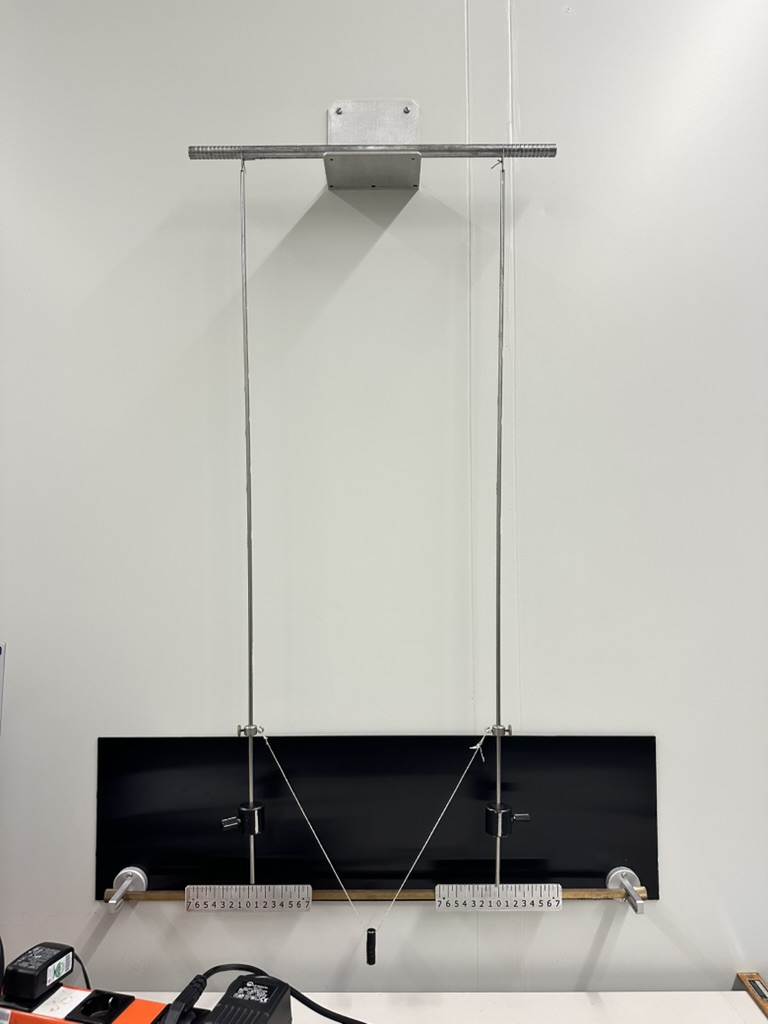
\includegraphics[width=0.4\textwidth]{Aufbau}}
	\caption{Aufbau der Pendel, die hier bei \(\lh = \qty{70}{\centi\meter}\) gekoppelt sind.}
	\label{fig:aufbau}
\end{figure}

Die Pendel werden durch lange, dünne Metallstäbe realisiert, die durch eine Fadenöse auf einem horizontal befestigten Metallstab gelagert sind, und auf deren Enden Gewichte gezogen und dann mit einer Schraube festgezogen werden können. Nach demselben Prinzip werden die Haken als Aufnahmepunkte für die Verbindung zwischen beiden Pendeln über den Gewichten installiert. Um die Pendel zu koppeln wird eine Schnur, die durch eine weitere Masse führt in die Haken eingehängt.

Von einer CCD-Kamera wird die Momentanauslenkung der Massen aufgezeichnet. Dafür sind an den Massen vertikal reflektierende Streifen angebracht. Der Fokus der Kamera wird auf \qty{0,9}{\meter} eingestellt. Die Blende wurde auf \num{11} eingestellt.

Mit einer Metallleiste, an der zwei verschiebbare Stopper angebracht sind, lassen sich die Pendel bestmöglich gleichphasig mit gleicher Amplitude auslenken. Um die gegensinnige Fundamentalschwingung zu erzeugen kann auch das Kopplungsgewicht nach unten gezogen werden.

Nach einer initialen Auslenkung wird im Messprogramm die Aufzeichnung gestartet und für ca. \qty{60}{\second} gemessen. Wird der Schwebungsfall gemessen, sollen mindestens \num{5} Minima abgewartet werden. Dann wird die Aufzeichnung gestoppt und durch Auswählen der interessanten Punkte im Diagramm die verstrichene Zeit mit der zugehörigen Anzahl an durchlaufenen Perioden notiert.



\section{Messwerte}

\begin{table}[H]
	\begin{tabular*}{\textwidth}{@{\extracolsep{\fill}}@{\hspace{5pt}}lrr@{\hspace{5pt}}}
		\toprule
		Parameter & Pendel \num{1} & Pendel \num{2}\\
		\midrule
		\(m\)\,/\,\si{\kilogram} & \num{176,97e-3}   & \num{174,95e-3}\\
		\(m_{\text{H}}\)\,/\,\si{\kilogram} & \num{16,06e-3}   & \num{15,80e-3}\\
		\(m_{\text{St}}\) \,/\,\si{\kilogram} & \num{131,40e-3} & \num{131,27e-3}\\
		\(L\)\,/\, \si{\meter} & \num{0,804} & \num{0,800}\\
		\(\lh\) \,/\, \si{\meter} & \num{0,4} & \num{0,4}\\
		\(L_{\text{St}}\)\,/\, \si{\meter} & \num{0,87} & \num{0,87}\\
		\bottomrule
	\end{tabular*}
	\caption{Massen und Längen der zwei Pendel \label{tbl:dimensions}}
\end{table}

\(t_0\) und \(t_1\) stehen im ungekoppelten Fall, sowie im gekoppelten Fall für die Fundamentalschwingungen stets für Zeitpunkte, zwischen denen \num{20} Perioden durchlaufen wurden. Im Schwebungsfall sind mit \(t_i\) alle Zeiten vermerkt, zu der das Pendel stillsteht.

\newpage

Im Folgenden sind die Messwerte für die Position \(\lh = \qty{40}{\centi\meter}\) tabelliert.

\begin{table}[H]
	\begin{tabular*}{\textwidth}{@{\extracolsep{\fill}}@{\hspace{5pt}}lrr@{\hspace{5pt}}}
		\toprule
		Pendel & \(t_0\)\,/\,\(\si{\second}\) & \(t_1\)\,/\,\(\si{\second}\)\\
		\midrule
		1 & \num{1,4}   & \num{35,5}\\
		2 & \num{1,3}   & \num{35,4}\\
		\bottomrule
	\end{tabular*}
	\caption{Ungekoppelter gleichsinniger Fall \label{tbl:ngekgl40}}
\end{table}

\begin{table}[H]
	\begin{tabular*}{\textwidth}{@{\extracolsep{\fill}}@{\hspace{5pt}}lrr@{\hspace{5pt}}}
		\toprule
		Pendel & \(t_0\)\,/\,\(\si{\second}\) & \(t_1\)\,/\,\(\si{\second}\)\\
		\midrule
		1 & \num{0,9}   & \num{34,8}\\
		2 & \num{0,8}   & \num{34,8}\\
		\bottomrule
	\end{tabular*}
	\caption{Gekoppelter gleichsinniger Fall \label{tbl:gekgl40}}
\end{table}

\begin{table}[H]
	\begin{tabular*}{\textwidth}{@{\extracolsep{\fill}}@{\hspace{5pt}}lrr@{\hspace{5pt}}}
		\toprule
		Pendel & \(t_0\)\,/\,\(\si{\second}\) & \(t_1\)\,/\,\(\si{\second}\)\\
		\midrule
		1 & \num{0,4}   & \num{33,3}\\
		2 & \num{1,2}   & \num{34,1}\\
		\bottomrule
	\end{tabular*}
	\caption{Gekoppelter gegensinniger Fall \label{tbl:gekgeg40}}
\end{table}

\begin{table}[H]
	\begin{tabular*}{\textwidth}{@{\extracolsep{\fill}}@{\hspace{5pt}}lrrrrr@{\hspace{5pt}}}
		\toprule
		Pendel & \(t_0\)\,/\,\(\si{\second}\) & \(t_1\)\,/\,\(\si{\second}\)& \(t_2\)\,/\,\(\si{\second}\)& \(t_3\)\,/\,\(\si{\second}\)& \(t_4\)\,/\,\(\si{\second}\)\\
		\midrule
		1 & \num{0,0}   & \num{52,4} & \num{105,8} & \num{160,0} & \num{211,6}\\
		2 & \num{25,4}   & \num{79,5} & \num{132,9} & \num{185,3} & \num{237,8}\\
		\bottomrule
	\end{tabular*}
	\caption{Schwebungsfall \label{tbl:schweb40}}
\end{table}

\newpage

Im Folgenden sind die Messwerte für die Position \(\lh = \qty{55}{\centi\meter}\) tabelliert.

\begin{table}[H]
	\begin{tabular*}{\textwidth}{@{\extracolsep{\fill}}@{\hspace{5pt}}lrr@{\hspace{5pt}}}
		\toprule
		Pendel & \(t_0\)\,/\,\(\si{\second}\) & \(t_1\)\,/\,\(\si{\second}\)\\
		\midrule
		1 & \num{0,8}   & \num{35,0}\\
		2 & \num{0,8}   & \num{34,8}\\
		\bottomrule
	\end{tabular*}
	\caption{Ungekoppelter gleichsinniger Fall \label{tbl:ngekgl55}}
\end{table}

\begin{table}[H]
	\begin{tabular*}{\textwidth}{@{\extracolsep{\fill}}@{\hspace{5pt}}lrr@{\hspace{5pt}}}
		\toprule
		Pendel & \(t_0\)\,/\,\(\si{\second}\) & \(t_1\)\,/\,\(\si{\second}\)\\
		\midrule
		1 & \num{0,5}   & \num{34,5}\\
		2 & \num{0,5}   & \num{34,5}\\
		\bottomrule
	\end{tabular*}
	\caption{Gekoppelter gleichsinniger Fall \label{tbl:gekgl55}}
\end{table}

\begin{table}[H]
	\begin{tabular*}{\textwidth}{@{\extracolsep{\fill}}@{\hspace{5pt}}lrr@{\hspace{5pt}}}
		\toprule
		Pendel & \(t_0\)\,/\,\(\si{\second}\) & \(t_1\)\,/\,\(\si{\second}\)\\
		\midrule
		1 & \num{1,4}   & \num{33,6}\\
		2 & \num{0,6}   & \num{32,9}\\
		\bottomrule
	\end{tabular*}
	\caption{Gekoppelter gegensinniger Fall \label{tbl:gekgeg55}}
\end{table}

\begin{table}[H]
	\begin{tabular*}{\textwidth}{@{\extracolsep{\fill}}@{\hspace{5pt}}lrrrrr@{\hspace{5pt}}}
		\toprule
		Pendel & \(t_0\)\,/\,\(\si{\second}\) & \(t_1\)\,/\,\(\si{\second}\)& \(t_2\)\,/\,\(\si{\second}\)& \(t_3\)\,/\,\(\si{\second}\)& \(t_4\)\,/\,\(\si{\second}\)\\
		\midrule
		1 & \num{14,8}   & \num{44,9} & \num{74,6} & \num{105,2} & \num{134,8}\\
		2 & \num{0,0}   & \num{29,5} & \num{60,2} & \num{89,8} & \num{119,6}\\
		\bottomrule
	\end{tabular*}
	\caption{Schwebungsfall \label{tbl:schweb55}}
\end{table}

\newpage

Im Folgenden sind die Messwerte für die Position \(\lh = \qty{70}{\centi\meter}\) tabelliert.

\begin{table}[H]
	\begin{tabular*}{\textwidth}{@{\extracolsep{\fill}}@{\hspace{5pt}}lrr@{\hspace{5pt}}}
		\toprule
		Pendel & \(t_0\)\,/\,\(\si{\second}\) & \(t_1\)\,/\,\(\si{\second}\)\\
		\midrule
		1 & \num{1,5}   & \num{35,8}\\
		2 & \num{1,5}   & \num{35,7}\\
		\bottomrule
	\end{tabular*}
	\caption{Ungekoppelter gleichsinniger Fall \label{tbl:ngekgl70}}
\end{table}

\begin{table}[H]
	\begin{tabular*}{\textwidth}{@{\extracolsep{\fill}}@{\hspace{5pt}}lrr@{\hspace{5pt}}}
		\toprule
		Pendel & \(t_0\)\,/\,\(\si{\second}\) & \(t_1\)\,/\,\(\si{\second}\)\\
		\midrule
		1 & \num{0,5}   & \num{34,7}\\
		2 & \num{0,5}   & \num{34,7}\\
		\bottomrule
	\end{tabular*}
	\caption{Gekoppelter gleichsinniger Fall \label{tbl:gekgl70}}
\end{table}

\begin{table}[H]
	\begin{tabular*}{\textwidth}{@{\extracolsep{\fill}}@{\hspace{5pt}}lrr@{\hspace{5pt}}}
		\toprule
		Pendel & \(t_0\)\,/\,\(\si{\second}\) & \(t_1\)\,/\,\(\si{\second}\)\\
		\midrule
		1 & \num{1,5}   & \num{33,0}\\
		2 & \num{0,7}   & \num{32,2}\\
		\bottomrule
	\end{tabular*}
	\caption{Gekoppelter gegensinniger Fall \label{tbl:gekgeg70}}
\end{table}

\begin{table}[H]
	\begin{tabular*}{\textwidth}{@{\extracolsep{\fill}}@{\hspace{5pt}}lrrrrr@{\hspace{5pt}}}
		\toprule
		Pendel & \(t_0\)\,/\,\(\si{\second}\) & \(t_1\)\,/\,\(\si{\second}\)& \(t_2\)\,/\,\(\si{\second}\)& \(t_3\)\,/\,\(\si{\second}\)& \(t_4\)\,/\,\(\si{\second}\)\\
		\midrule
		1 & \num{0,0}   & \num{18,1} & \num{38,7} & \num{58,3} & \num{77,8}\\
		2 & \num{9,0}   & \num{29,5} & \num{49,0} & \num{68,6} & \num{88,3}\\
		\bottomrule
	\end{tabular*}
	\caption{Schwebungsfall \label{tbl:schweb70}}
\end{table}

\begin{table}[H]
	\begin{tabular*}{\textwidth}{@{\extracolsep{\fill}}@{\hspace{5pt}}lrrrrr@{\hspace{5pt}}}
		\toprule
		Pendel & \(t_0\)\,/\,\(\si{\second}\) & \(t_1\)\,/\,\(\si{\second}\)& \(t_2\)\,/\,\(\si{\second}\)& \(t_3\)\,/\,\(\si{\second}\)& \(t_4\)\,/\,\(\si{\second}\)\\
		\midrule
		1 & \num{6,2}   & \num{26,7} & \num{47,1} & \num{66,9} & \num{85,6}\\
		2 & \num{16,4}   & \num{36,9} & \num{57,3} & \num{77,1} & \num{97,4}\\
		\bottomrule
	\end{tabular*}
	\caption{Schwebungsfall für unterschiedlich ausgelenkte Massen \label{tbl:schwebX70}}
\end{table}

\section{Auswertung}

\(T_0\) berechnet sich aus den Daten, die in \autoref{tbl:ngekgl40} eingetragen sind durch
\begin{equation}
	T_0 = \frac{t_1 - t_0}{20} = \frac{\qty{35,5}{\second} - \qty{1,4}{\second}}{20} = \qty{1,7}{\second} \,.
\end{equation}
Für Pendel \num{2} folgt analog ebenfalls \(T_0 =\qty{1,7}{\second}\). Somit ist dies auch das Mittel. Dieses Prinzip wird auf alle \(T_{\text{gl}}\) und \(T_{\text{geg}}\) angewendet.

\(T_{\text{II}}\) wird durch \autoref{eq:t2} ermittelt. %Inline Equation Link

Bei \(T_{\text{S}}\) wird der erste und der letzte Zeitpunkt des Stillstandes des Pendel, der in der Messdauer liegt auf die Anzahl der Schwebungsdauern in diesem Intervall normiert. %Wording?!

Für die entsprechenden Kopplungsgrade ergeben sich die folgende Periodendauern.

\begin{table}[H]
	\begin{tabular*}{\textwidth}{@{\extracolsep{\fill}}@{\hspace{5pt}}lrrr@{\hspace{5pt}}}
		\toprule
		Periodendauer & Links & Rechts & Mittel\\
		\midrule
		\(T_{\text{gl}}\) & \qty{1,7}{\second} & \qty{1,7}{\second} & \qty{1,7}{\second}\\
		\(T_{\text{geg}}\) & \qty{1,6}{\second} & \qty{1,6}{\second} & \qty{1,6}{\second}\\
		\(T_{\text{II}}\) & \qty{1,6}{\second} & \qty{1,6}{\second} & \qty{1,6}{\second}\\
		\(T_{\text{S}}\) & \qty{52,9}{\second} & \qty{53,1}{\second} & \qty{53,0}{\second} \\
		\bottomrule
	\end{tabular*}
	\caption{Periodendauern für \(\lh = \qty{40}{\centi\meter}\) \label{tbl:res40}}
\end{table}


\begin{table}[H]
	\begin{tabular*}{\textwidth}{@{\extracolsep{\fill}}@{\hspace{5pt}}lrrr@{\hspace{5pt}}}
		\toprule
		Periodendauer & Links & Rechts & Mittel\\
		\midrule
		\(T_{\text{gl}}\) & \qty{1,7}{\second} & \qty{1,7}{\second} & \qty{1,7}{\second}\\
		\(T_{\text{geg}}\) & \qty{1,6}{\second} & \qty{1,6}{\second} & \qty{1,6}{\second}\\
		\(T_{\text{II}}\) & \qty{1,6}{\second} & \qty{1,6}{\second} & \qty{1,6}{\second}\\
		\(T_{\text{S}}\) & \qty{30,0}{\second} & \qty{29,9}{\second} & \qty{30,0}{\second} \\
		\bottomrule
	\end{tabular*}
	\caption{Periodendauern für \(\lh = \qty{55}{\centi\meter}\) \label{tbl:res55}}
\end{table}

\begin{table}[H]
	\begin{tabular*}{\textwidth}{@{\extracolsep{\fill}}@{\hspace{5pt}}lrrr@{\hspace{5pt}}}
		\toprule
		Periodendauer & Links & Rechts & Mittel\\
		\midrule
		\(T_{\text{gl}}\) & \qty{1,7}{\second} & \qty{1,7}{\second} & \qty{1,7}{\second}\\
		\(T_{\text{geg}}\) & \qty{1,6}{\second} & \qty{1,6}{\second} & \qty{1,6}{\second}\\
		\(T_{\text{II}}\) & \qty{1,6}{\second} & \qty{1,6}{\second} & \qty{1,6}{\second}\\
		\(T_{\text{S}}\) & \qty{19,5}{\second} & \qty{19,8}{\second} & \qty{19,6}{\second} \\
		\(\tilde{T}_{\text{S}}\) & \qty{19,9}{\second} & \qty{20,3}{\second} & \qty{20,1}{\second}\\
		\bottomrule
	\end{tabular*}
	\caption{Periodendauern für \(\lh = \qty{70}{\centi\meter}\) \label{tbl:res70}. \(\tilde{T}_{\text{S}}\) sind die Schwebungsdauern die gemessen wurden, als die Schwebung durch ungleiche Auslenkungen erzeugt wurde.}
\end{table}


\begin{figure}[H]
	\centering{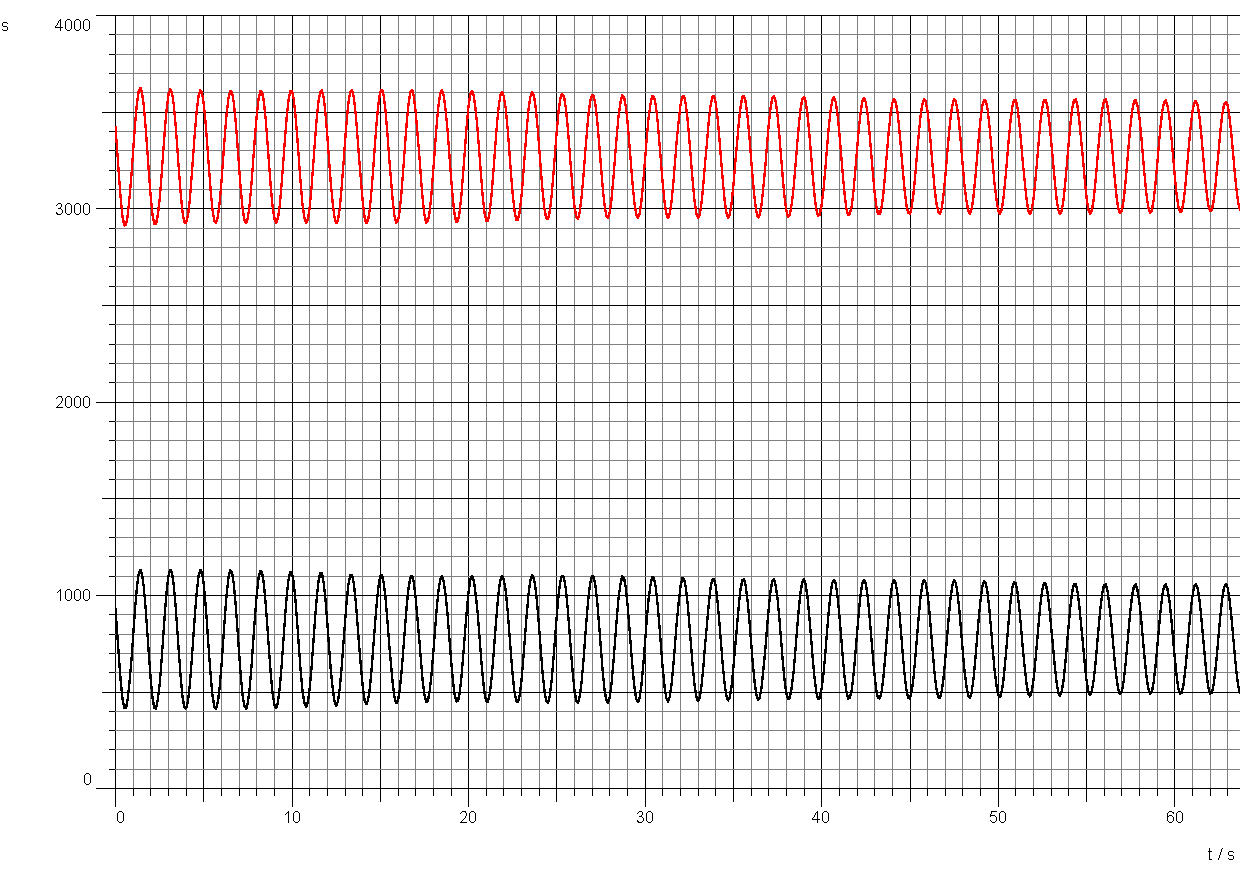
\includegraphics[width=0.7\textwidth]{gleichsinnige_FUNDAMENTALSCHWINGUNG_70cm.pdf}}
	\caption{Exemplarisches \(x(t)\)-Diagramm der gleichsinnigen Fundamentalschwingung bei \(\lh = \qty{70}{\centi\meter}\)}
	\label{fig:gl70}
\end{figure}

\begin{figure}[H]
	\centering{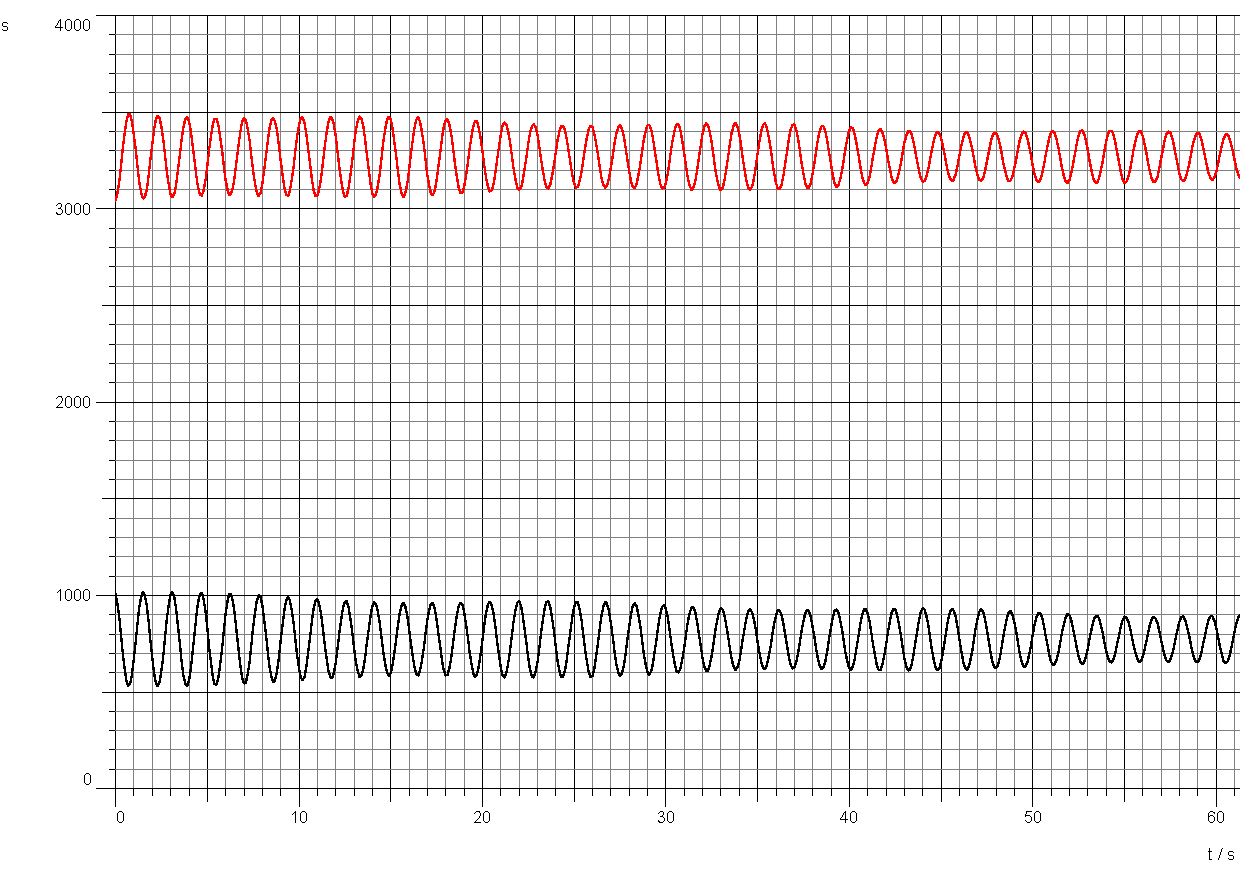
\includegraphics[width=0.7\textwidth]{gegensinnige_FUNDAMENTALSCHWINGUNG_70cm.pdf}}
	\caption{Exemplarisches \(x(t)\)-Diagramm der gegensinnigen Fundamentalschwingung bei \(\lh = \qty{70}{\centi\meter}\)}
	\label{fig:geg70}
\end{figure}

\begin{figure}[H]
	\centering{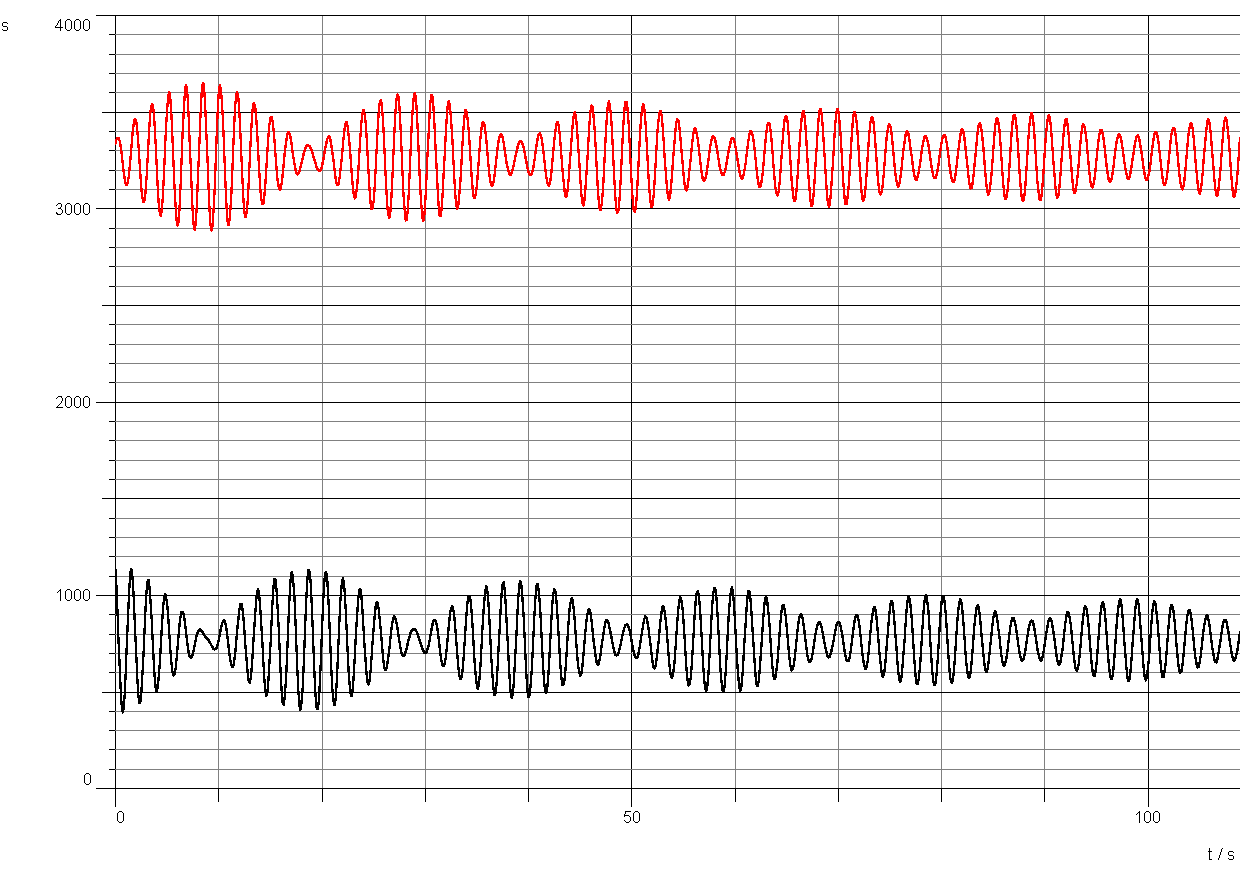
\includegraphics[width=0.7\textwidth]{SCHWEBUNG_70cm.pdf}}
	\caption{Exemplarisches \(x(t)\)-Diagramm des Schwebungsfalles bei \(\lh = \qty{70}{\centi\meter}\)}
	\label{fig:schweb}
\end{figure}

\begin{figure}[H]
	\centering{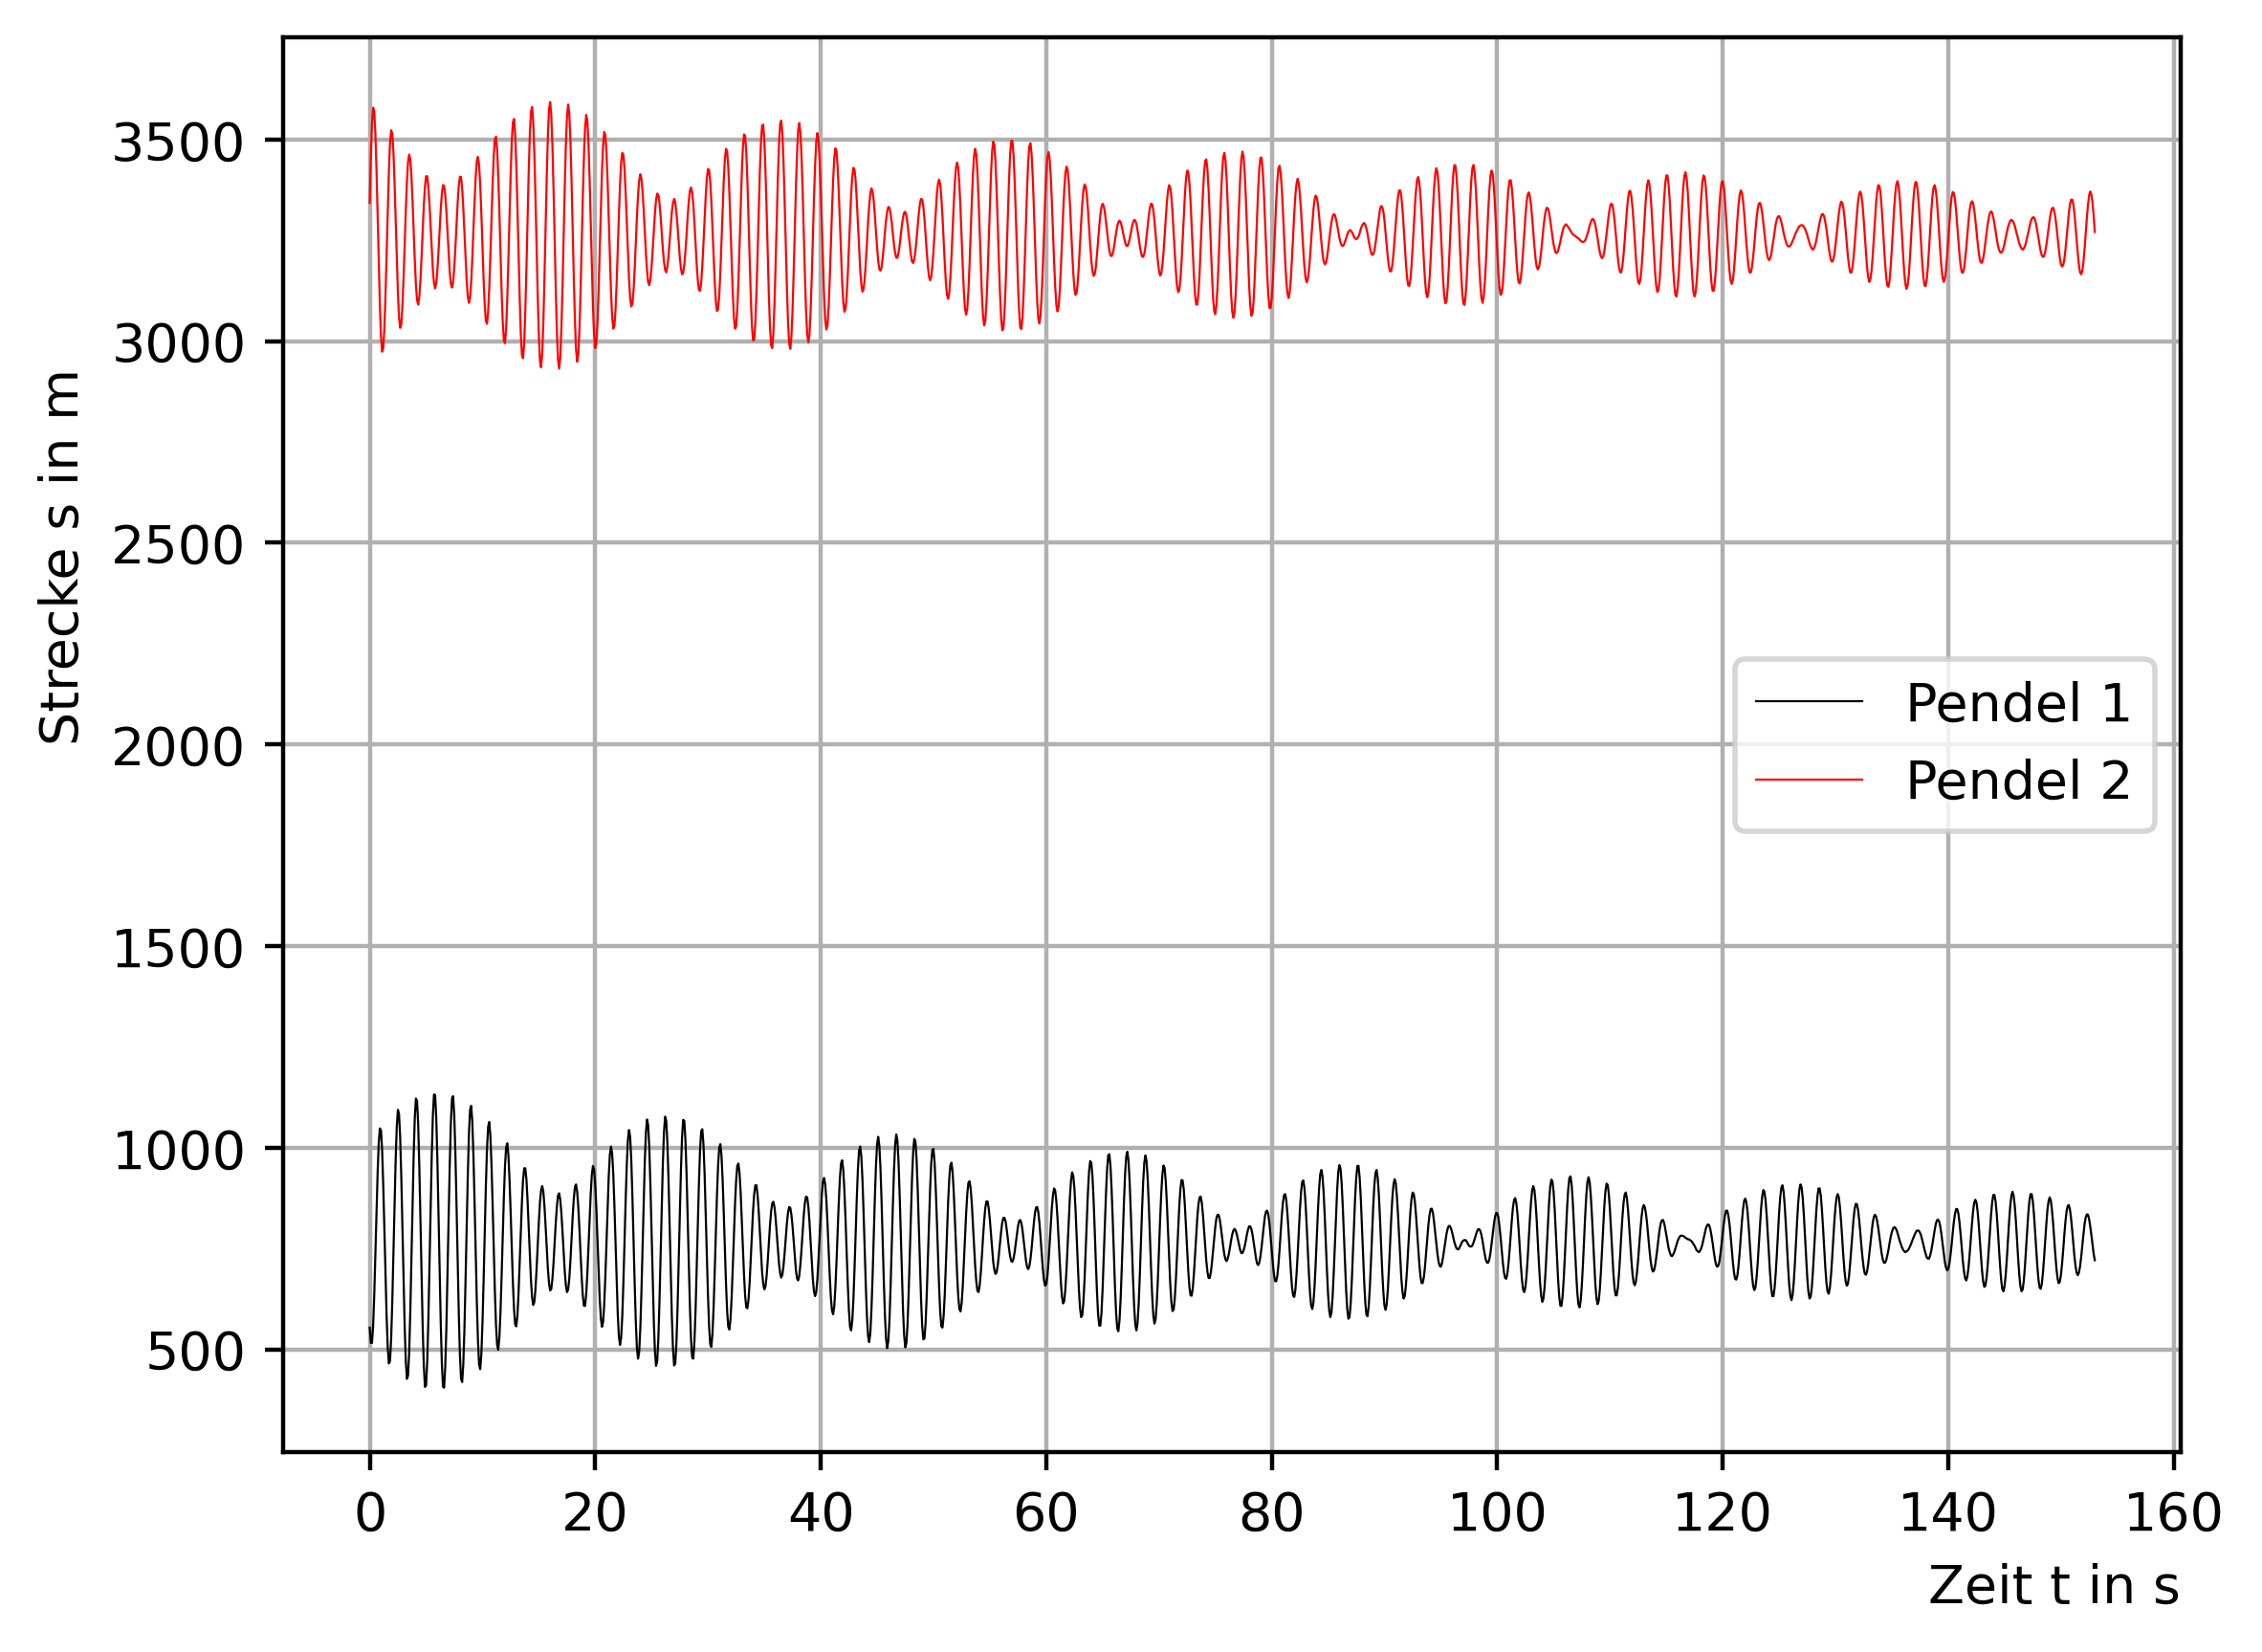
\includegraphics[width=0.75\textwidth]{ungleicherSchweb.png}}
	\caption{Exemplarisches \(x(t)\)-Diagramm der gegensinnigen Fundamentalschwingung bei \(\lh = \qty{70}{\centi\meter}\)}
	\label{fig:ungl70}
\end{figure}

Wie aus \autoref{tbl:res70} hervorgeht, liegen \(T_{\text{S}}\) und \(\tilde{T}_{\text{S}}\) sehr nah beieinander. Daran lässt sich sehen, dass die Schwebungsdauer nicht davon abhängt, ob nur ein Pendel oder beide -- dann aber unterschiedlich -- ausgelenkt werden. Dies liegt daran, dass die Schwebungsdauer nur von den Eigenfrequenzen des Systems abhängt, und diese ändern sich nicht, solange man die Dimensionen des Systems nicht manipuliert.

%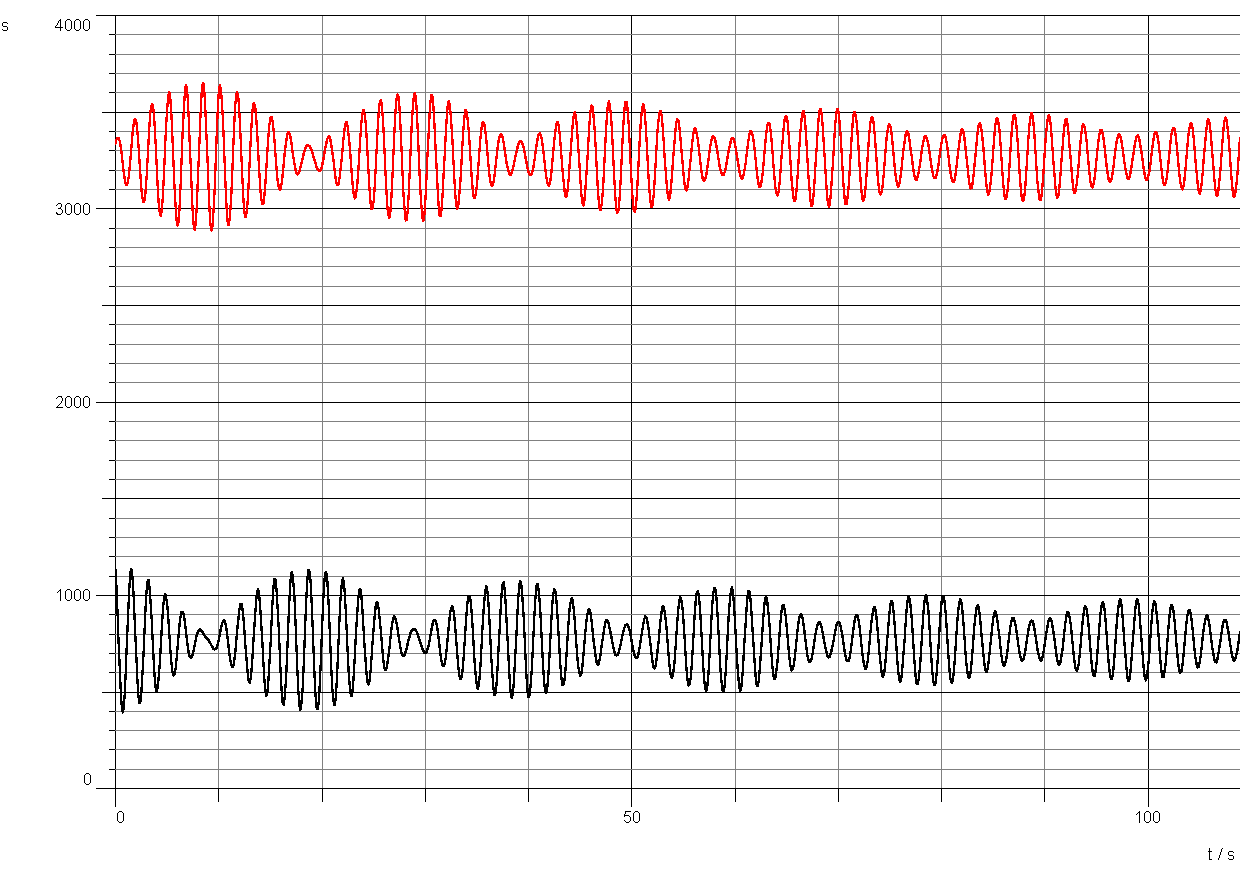
\includepdf[pages=-]{SCHWEBUNG_70cm.pdf}
%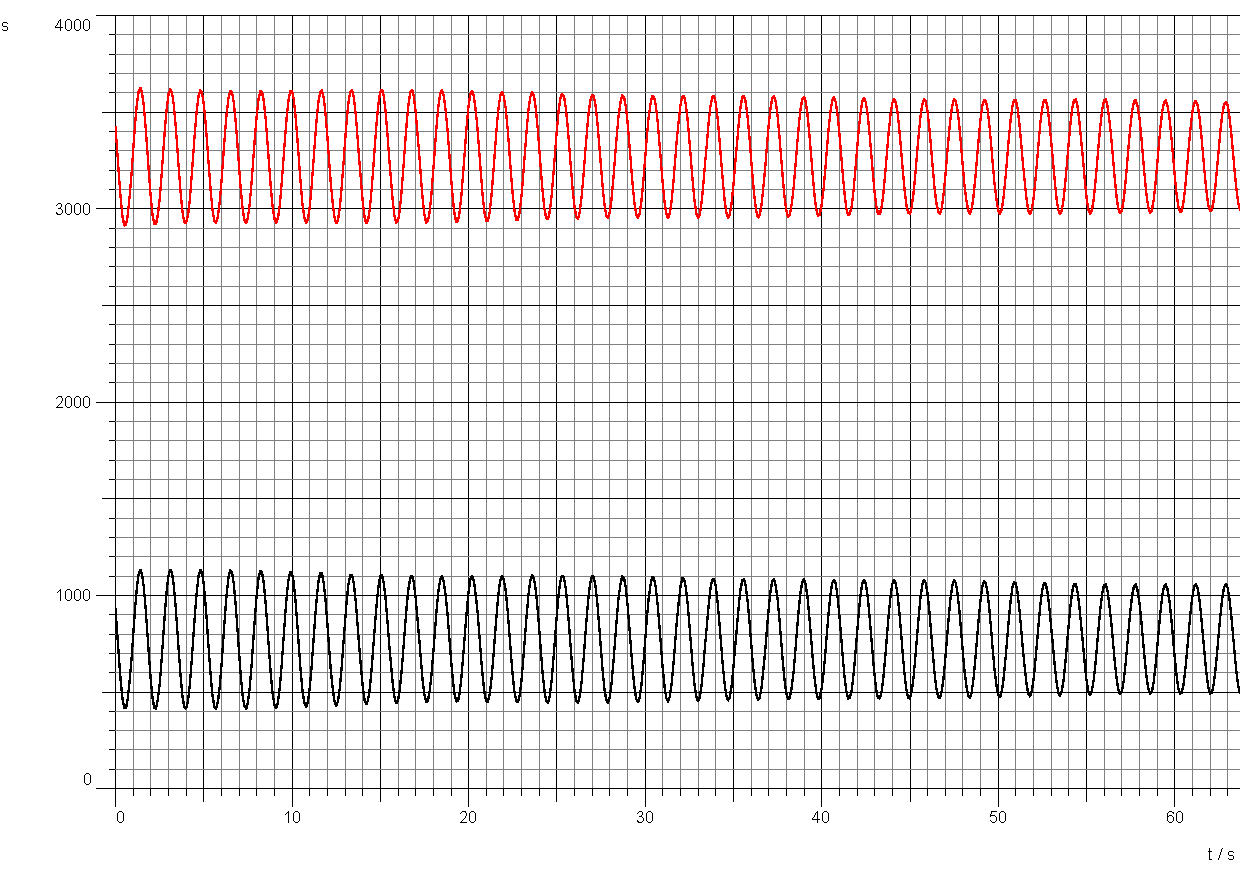
\includepdf[pages=-]{gleichsinnige_FUNDAMENTALSCHWINGUNG_70cm.pdf}
%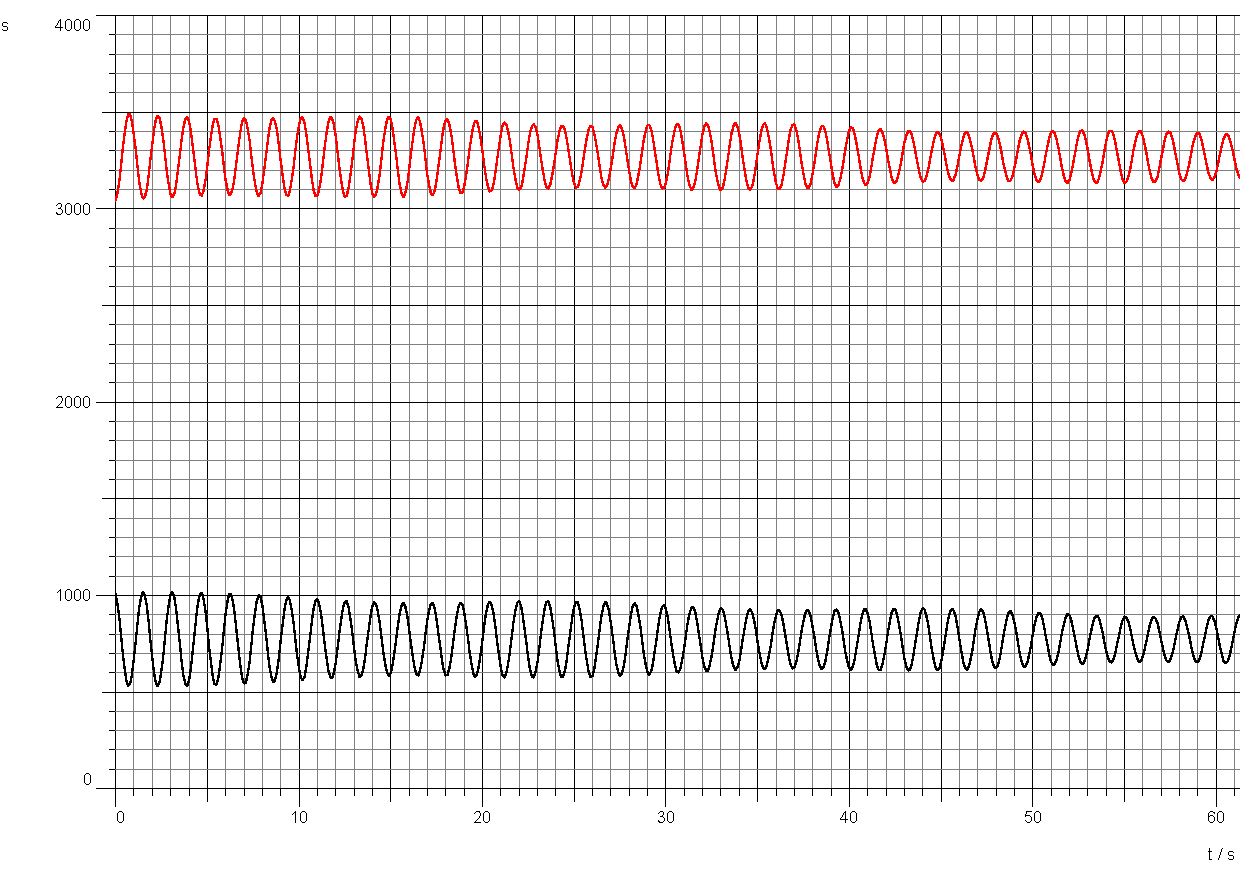
\includepdf[pages=-]{gegensinnige_FUNDAMENTALSCHWINGUNG_70cm.pdf}

Nach \autoref{eq:trägheitsmom} wird das Gesamtträgheitsmoment mit den Daten aus \autoref{tbl:dimensions} berechnet. Für das erste Pendel ergibt sich das Trägheitsmoment
\begin{equation}
	\begin{split}
		J_1 = \frac{1}{3} \cdot \qty{131,40e-3}{\kilogram} \cdot (\qty{0,87}{\meter})^2 &+ \qty{16,06e-3}{\kilogram} \cdot (\qty{0,4}{\meter})^2
		\\&+ \qty{176,97e-3}{\kilogram} \cdot (\qty{0,804}{\meter})^2 = \qty{0,150}{\kilogram\meter\squared}
	\end{split}
\end{equation}
und für das zweite Pendel \(J_2 = \qty{0,148}{\kilogram\meter\squared}\).

Die Eigenfrequenz \(\omega_0\) wird mittels \autoref{eq:eig} %Der Link ist komisch
berechnet. Dafür muss zuerst die Lage des Schwerpunktes \(\ls\) mit %\autoref{eq:schwerp}
berechnet werden und ergibt
\begin{equation}
	\ls = \frac{Lm + \lh m_{\text{H}} + \tfrac{1}{2} L_{\text{St}} m_{\text{St}}}{m + m_{\text{H}} + m_{\text{St}}}
\end{equation}
\begin{equation}
	\begin{split}
		\ell_{\text{S},1} &= \frac{\qty{0,804}{\meter} \cdot \qty{176,97e-3}{\kilogram} + \qty{0,4}{\meter} \cdot \qty{16,06e-3}{\kilogram} + \tfrac{1}{2}\qty{0,87}{\meter} \cdot \qty{131,40e-3}{\kilogram}}{\mleft(\num{176,97e-3} + \num{16,06e-3} + \num{131,40e-3}\mright)\si{\kilogram}}\\
		&= \qty{0,635}{\meter}
	\end{split}
\end{equation}
Für \(\ell_{\text{S},2}\) ergibt sich \(\ell_{\text{S},1} = \qty{0,632}{m}\). Die Schwerpunktmasse des erten Pendels \(M_1\) ist
\begin{equation}
	\begin{split}
		M_1 &= m_1 + m_{\text{H},1} + m_{\text{St},1}\\
		&= \qty{176,97e-3}{\kilogram} + \qty{16,06e-3}{\kilogram} + \qty{131,40e-3}{\kilogram}\\
		&= \qty{324,43e-3}{\kilogram} \,.
	\end{split}
\end{equation}
Für das zweite Pendel ist \(M_2 = \qty{322,02e-3}{\kilogram}\). Damit beläuft sich die Eigenfrequenz \(\omega_{0,1}\) auf
\begin{equation}
	\omega_{0,1} = \sqrt{\frac{M_1 g \ls}{J_1}} = \sqrt{\frac{\qty{324,43e-3}{\kilogram} \cdot \qty{9,81}{\meter\per\second\squared} \cdot \qty{0,635}{\meter}}{\qty{0,150}{\kilogram\meter\squared}}} = \qty{3,671}{\hertz} \,.
\end{equation}
Folgerichtig gilt \(\omega_{0,2} = \qty{3,673}{\hertz}\).

Aus den gemessenen Größen ergeben sich die gemessenen Eigenfrequenzen
\begin{equation}
	\omega_{0,1} = \frac{2\pi}{\qty{1,7}{\second}} = = \qty{3,7}{\hertz}
\end{equation}
und \(\omega_{0,2} = \qty{3,7}{\hertz}\).

\begin{table}[H]
	\begin{tabular*}{\textwidth}{@{\extracolsep{\fill}}@{\hspace{5pt}}lrr@{\hspace{5pt}}}
		\toprule
		Länge & \(K\) nach \autoref{eq:2} & \(K\) nach \autoref{eq:3}\\
		\midrule
		\(\lh = \qty{40}{\centi\meter}\) & \num{0,0606} & \num{0,0302}\\
		\(\lh = \qty{55}{\centi\meter}\) & \num{0,0606} & \num{0,0533}\\
		\(\lh = \qty{70}{\centi\meter}\) & \num{0,0606} & \num{0,0815}\\
		\bottomrule
	\end{tabular*}
	\caption{Kopllungsgrade berechnet durch verschiedene Gleichungen. \label{tbl:kopplungsgrade}}
\end{table}


%\section{Fehlerrechnung}

\section{Zusammenfassung}
Die Kopplungsgrade verändern sich nur geringfügig. Dabei sollte \autoref{eq:2} die genaueren Ergebnisse liefern, da er mit den direkt gemessenen Periodendauern berechnet werden kann, während bei \autoref{eq:3} mehrere Messungen und Rechnungen für $T_{\text{II}}$ nötig sind, wodurch größere Unsicherheiten das Ergebnis verfälschen.

\begin{thebibliography}{999}
	\bibitem{Quelle} Versuchsanleitung zu \emph{M23 -- Gekoppelte Pendel} (Abgerufen am 25.09.2025)
\end{thebibliography}


\section{Anhang}

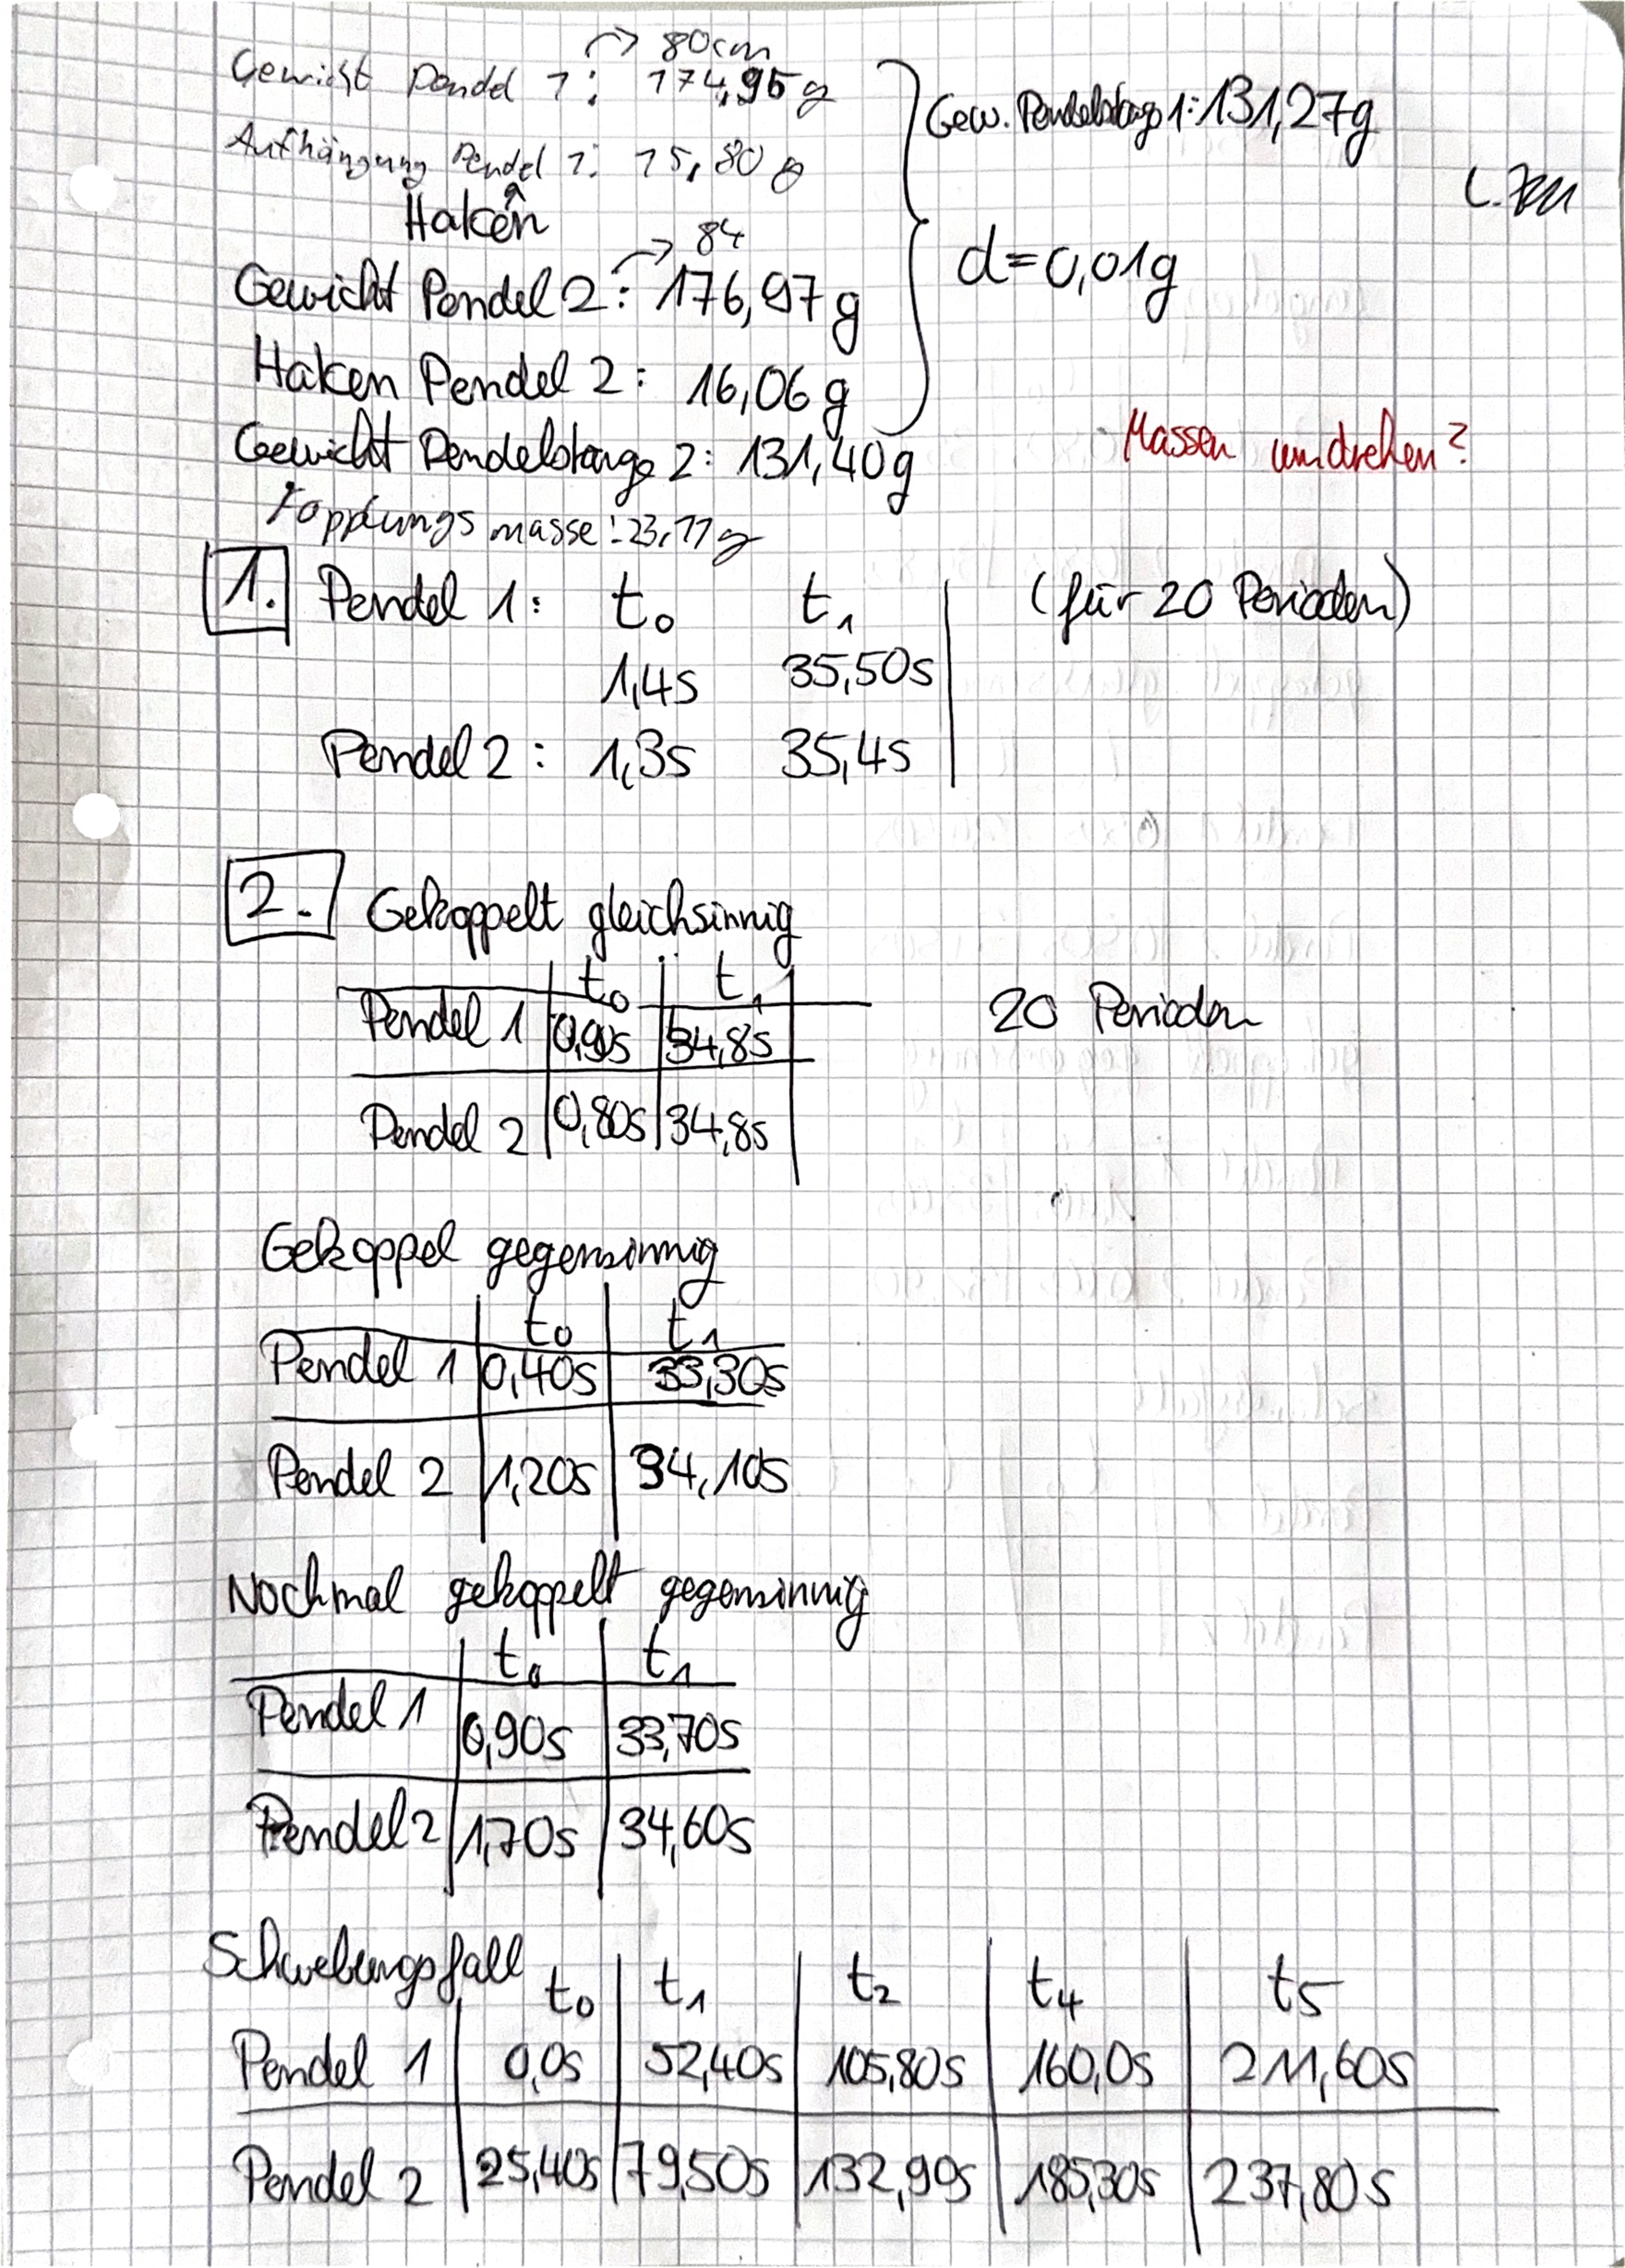
\includepdf[pages=-]{Messprotokoll.pdf}

\end{document}